\documentclass{beamer}
\usepackage{pgffor,pgfmath}
\usepackage{lipsum}
\usepackage{multicol}
\usetheme{ucla}
\usepackage{graphicx}
\usepackage{listings}
\usepackage{verbatim}
\usepackage{tikz}
\linespread{1.5}
\usepackage{comment}

\usepackage{amsmath, amsthm, amssymb, latexsym}

%\newtheorem{definition}{Definition}

\title{Lecture 4}
\author{Charles Rambo}
\institute{UCLA Anderson School of Management}
\date{2023}
\location{Los Angeles, California}

% Turn on slide numbers:
\showSlideNumber{}

\AtBeginSection[]
{
    \begin{frame}
        \frametitle{Table of Contents}
        \tableofcontents[currentsection]
    \end{frame}
}


\begin{document}

\insertTitleSlide

\section{Linear Algebra}
\subsection{Vector Spaces}

\begin{frame}
\frametitle{Vector Spaces}
\begin{Definition}
A {\bf real vector space} $V$ is a set such that--for $u$, $v$, and $w$ in $V$ and $\alpha$ and $\beta$ in $\mathbb{R}$--the following hold.
{
\small
\begin{multicols}{2}
\begin{enumerate}
\item[VS.1] $(u + v) + w = u + (v + w)$.
\item[VS.2] There is an element $O$ in $V$ such that
$$
O + u = u + O = u.
$$
\item[VS.3] There exists $-u$ in $V$ such that
$$
u + (-u) = (-u) + u = O.
$$
\item[VS.4] $u + v = v + u$.
\item[VS.5] $\alpha(u + v) = \alpha u + \alpha v$.
\item[VS.6] $(\alpha + \beta) u = \alpha u + \beta u$.
\item[VS.7] $(\alpha\beta) u = \alpha(\beta u)$.
\item[VS.8] $1 u = u$.
\end{enumerate}
\end{multicols}
}
\end{Definition}
\end{frame}

\begin{frame}
\frametitle{Subspaces}
\begin{Definition}
Let $V$ be a vector space and let $W$ be a subset of $V$. Then $W$ is a {\bf subspace} of $V$ if the following properties hold.
\begin{enumerate}
\item[(a)] $w_1$ and $w_2$ in $W$ implies $w_1 + w_2$ is in $W$
\item[(b)] $\alpha$ in $\mathbb{R}$ and $w$ in $W$ implies $\alpha w$ is in $W$
\item[(c)] The element $O$ is in $W$
\end{enumerate}
\end{Definition}

\end{frame}

\begin{frame}
\frametitle{Vector Spaces and Subspaces}
\begin{Example}
The set $V = \{f:\mathbb{R}\to\mathbb{R}| f\ \text{continuous}\}$ is a real vector space and $W = \{f:\mathbb{R}\to\mathbb{R}| f\ \text{differentiable}\}$ is a subspace, if for $f$ and $g$ in $V$, we define $f + g$ to be the function which satisfies 
$$
(f + g)(x) = f(x) + g(x)
$$
and $\alpha$ in $\mathbb{R}$ we define $\alpha f$ to be the function which satisfies 
$$
(\alpha f)(x) = \alpha f(x).
$$
\end{Example}
\end{frame}

\begin{frame}
\frametitle{Linear Independence}
\begin{Definition}
Let $\{v_1, v_2,\ldots, v_n\}$ to be a set of elements of $V$. Then the set is {\bf linearly independent} if for $\alpha_1, \alpha_2,\ldots, \alpha_n$ in $\mathbb{R}$, 
$$
\alpha_1 v_1 + \alpha_2 v_2+\ldots + \alpha_n v_n = O\qquad\text{implies}\qquad \alpha_i = 0\ \text{for all}\ i.
$$
If the set is not linearly independent, then it is {\bf linearly dependent}. 
\end{Definition}

\end{frame}

\begin{frame}
\frametitle{Span}
\begin{Definition}
The {\bf span} of $\{v_1, v_2,\ldots, v_m\}$ is 
$$
\text{span}\{v_1, v_2,\ldots, v_m\} = \{\alpha_1v_1 + \alpha_2 v_2 + \ldots + \alpha_m v_m : \alpha_i\in\mathbb{R}\}.
$$
\end{Definition}
\end{frame}

\begin{frame}
\frametitle{Basis}
\begin{Definition}
The set $\{v_1, v_2,\ldots, v_n\}$ is a {\bf basis} of $V$ if
\begin{enumerate}
\item[(a)] $\text{span}\{v_1, v_2,\ldots, v_n\} = V$ and
\item[(b)] The set $\{v_1, v_2,\ldots, v_n\}$ is linearly independent.
\end{enumerate}
\end{Definition}
\end{frame}

\begin{frame}
\frametitle{Standard Basis}
Consider $\mathbb{R}^n$ as a real vector space. If we define
\begin{align*}
e_1 	&= (1, 0, \ldots, 0, 0)\\
e_2 	&= (0, 1, \ldots, 0, 0)\\
	&\ \ \vdots\\
e_{n - 1} &= (0, 0, \ldots, 1, 0)\\
e_n &= (0, 0, \ldots, 0, 1),
\end{align*}
then $\{e_1, e_2, \ldots, e_{n - 1}, e_n\}$ is a basis for $\mathbb{R}^n$.
\end{frame}

\begin{frame}
\frametitle{Basis Elements and Dimension}
\begin{Theorem}
Let $V$ be a vector space. Let $\{v_1, v_2,\ldots, v_m\}$ be a basis of $V$. Suppose $w_1, w_2, \ldots w_n$ are elements fo $V$ and assume $n > m$. Then $w_1, w_2,\ldots, w_n$ are linearly dependent.
\end{Theorem}
\begin{Theorem}
Suppose $V$ is a vector space. If one basis has $m$ elements, and another has $n$ elements, then $m = n$.
\end{Theorem}
This means that the number of elements in a basis is unique. 
\begin{Definition}
The {\bf dimension} of a vector space $V$ is the number of elements in any basis of $V$.
\end{Definition}
\end{frame}

\subsection{Matrices} 

\begin{frame}[t]
\frametitle{Matrix Arithmetic}
\begin{Example}
Suppose 
$$
A = \left(\begin{array}{c c c} 1	&	2	&	3\\	-1	&	0	&	2\end{array}\right)\qquad\text{and}\qquad B = \left(\begin{array}{c c c} -1	&	5	&	-2\\	2	&	2	&	-1\end{array}\right).
$$
Compute (a) $2 A + B$ and (b) $A B^T$.
\end{Example}

\end{frame}

\begin{frame}
\frametitle{Python Matrix Arithmetic}
\begin{Example}
Suppose
$$
C = \left(\begin{array}{c c c c} 2		& 	1	&	3	&	4\\	-3	&	1	&	5	&	1\\	5	&	-1	&	11	&	7\\	-1	&	10	&	2	&4 \end{array}\right)
\qquad\text{and}\qquad
D =  \left(\begin{array}{c c c c} 100	& 	-5	&	2	&	1\\	7	&	-2	&	1	&	1\\	-5	&	1	&	2	&	3\\	20	&	1	&	4	&	50 \end{array}\right).
$$
Use Python to compute (a) $2C + D$ and (b) $C D^T$.
\end{Example}

\end{frame}

\begin{frame}[fragile]
\frametitle{Python Matrix Arithmetic Cont.}
{\bf Solution.}  
{\tiny
\begin{verbatim*}
# Import module
import numpy as np

# Define matrices
C = np.array([[2, 1, 3, 4], [-3, 1, 5, 1], [5, -1, 11, 7], [-1, 10, 2, 4]])
D = np.array([[100, -5, 2, 1], [7, -2, 1, 1], [-5, 1, 2, 3], [20, 1, 4, 50]])

# Perform arithmetic 
result_a = 2 * C + D
result_b = C @ D.T
\end{verbatim*}

The results are
$$
\texttt{result\_a}  = \left(\begin{array}{c c c c} 104	&	-3	&	8	&	9\\	1	&	0	&	11	&	3\\ 5	&	-1	&	24	&	17\\	18	&	21	&	8	&	58 \end{array}\right)
\qquad\text{and}\qquad 
\texttt{result\_b}	= \left(\begin{array}{c c c c} 205	&	19	&	9	&	253\\	-294	&	-17	&	29	&	11\\ 534	&	55	&	17	&	493\\	-142	&	-21	&	31	&	198 \end{array}\right).
$$
}
\end{frame}

\begin{frame}
\frametitle{Special Matrices}
\begin{itemize} 
\item The $n\times n$ identity matrix $I$, such that $A I = A$ for $A$ an $m\times n$ matrix and $I B = B$ for $B$ an $n\times m$ matrix. This matrix has ones on the main diagonal and zeros elsewhere. In Python, the command for the $n\times n$ identity matrix is \texttt{np.eye(n)}.
\item If $A$ is an $n\times n$ {\bf invertible} or {\bf non-singular} matrix, there is an $n\times n$ matrix $B$ such that $AB = BA = I$. We typically call $B$ the {\bf inverse} of $A$ and write it as $A^{-1}$. In Python, the command is \texttt{np.linalg.inv(A)}.
\end{itemize}
\end{frame}

\begin{frame}
\frametitle{Useful Inverse Matrix Formula}
Suppose
$$
A = \left(\begin{array}{c c} a	& 	b\\	c	&	d\end{array}\right).
$$
Then
$$
A^{-1} = \frac{1}{ad -bc}\left(\begin{array}{c c}	d	&	-b\\	-c	&	a\end{array}\right)
$$
whenever the formula makes sense.
\end{frame}

\subsection{Linear Transformations}

\begin{frame}
\frametitle{Linear Transformations}
\begin{Definition}
Let $U$ and $V$ be real vector spaces, and suppose $\alpha$ and $\beta$ are in $\mathbb{R}$. A {\bf linear transformation} $T: U\to V$ satisfies 
$$
T(\alpha u_1 + \beta u_2) = \alpha T(u_1) + \beta T(u_2)
$$
for all $u_1$ and $u_2$ in $U$. The vector space $U$ is the {\bf domain} of $T$ and $V$ is the {\bf codomain} of $T$. The set $\text{Im}(T) = \{T(u) : u\in U\}$ is the {\bf image} or {\bf range} of $T$.
\end{Definition}

\end{frame}

\begin{frame}[t]
\frametitle{Example}
\begin{Example}
Prove $F: \mathbb{R}^3\to\mathbb{R}^2$ defined by $F:(x, y, z)\mapsto (x, y)$ is a linear transformation.
\end{Example}

\end{frame}

\begin{frame}
\frametitle{Kernel}
\begin{Definition}
The {\bf kernel} of a linear transformation $T:U\to V$ is 
$$
\text{Ker}(T) = \{u : T(u) = O\}.
$$
\end{Definition}
\end{frame}

\begin{frame}
\frametitle{Kernel Example}
\tiny
\begin{Example}
Define $T: \mathbb{R}^3\to \mathbb{R}^2$ via
$$
T\left(\begin{array}{c} x_1\\ x_2\\ x_3\end{array}\right) = \left(\begin{array}{c c c} -1	&	0	&	1\\  5		&	1	&	-5\end{array}\right) \left(\begin{array}{c} x_1\\ x_2\\ x_3\end{array}\right).
$$
Find $\text{Ker}(T)$.
\end{Example}

{\bf Solution.} Typically this is done by row reducing $A$. You can also use the function \texttt{scipy.linalg.null\_space}. In either case, the kernel is
$$
\text{Ker}(A) = \text{span}\left\{\left(\begin{array}{c} 1\\ 0\\ 1\end{array}\right)\right\}.
$$
\end{frame}

\begin{frame}
\frametitle{Kernel Theorems}
\begin{Theorem}
Suppose $T: U\to V$. The set $\text{Ker}(T)$ is a subspace of $U$.
\end{Theorem}

\begin{Theorem}[Rank-Nullity Theorem]
Let $U$ be a vector space. Let $T: U\to V$ be a linear transformation of $U$ into another vector space $V$. Then
$$
\text{dim}(U) = \underbrace{\text{dim\ Ker}(T)}_{nullity} + \overbrace{\text{dim\ Im}(T)}^{rank}
$$
\end{Theorem}

\end{frame}

\subsection{Coordinate and Matrix Representation} 

\begin{frame}
\frametitle{Coordinate Representation of a Vector}
For $V$ a vectors space with basis $\mathcal{B} = (v_1, v_2,\ldots, v_n)$. We can represent an arbitrary $w$ in $V$ using the unique linear combination of the elements of $\mathcal{B}$. Specifically, 
$$
w = \alpha_1 v_1 + \alpha_2 v_2 +\ldots \alpha_n v_n.
$$
Using this, we can write the coordinate representation of $w$ with respect to the basis $\mathcal{B}$:
$$
(w)_\mathcal{B} = \left(\begin{array}{c} \alpha_1\\ \alpha_2\\\vdots\\ \alpha_n\end{array}\right).
$$
\end{frame}

\begin{frame}
\frametitle{Linear Transformations and Matrices}
There is a matrix representation of any linear transformations between finite dimensional vector spaces. Consider vector space $U$ with ordered basis $\mathcal{B} = (u_1, u_2,\ldots, u_m)$, and vector space $V$ with ordered basis $\mathcal{C} = (v_1, v_2,\ldots, v_n)$. Suppose $T: U\to V$ such that
$$
T(u_j) = \alpha_{1 j} v_1 + \alpha_{2 j} v_2 + \ldots + \alpha_{nj} v_n.
$$
Then the matrix representation in terms of these two bases is
$$
\mathcal{M}(T)_{\mathcal{B}}^{\mathcal{C}} = \left(\begin{array}{c c c c} \alpha_{11}	&	\ldots	&	\alpha_{1m}\\
												
													\vdots	& \ddots	&	\vdots\\
												\alpha_{n1}	&	\ldots	&	\alpha_{nm}\end{array}\right).
$$
\end{frame}

\begin{frame}[t]
\frametitle{Linear Transformations and Matrices Example}
\begin{Example}
Consider $F:\mathbb{R}^3\to \mathbb{R}^2$ defined by $F(x, y, z) = (x, y)$. Write the matrix representation of $F$ in terms of the standard bases.
\end{Example}

\end{frame}

\begin{frame}
\frametitle{Change of Basis}
Suppose we have bases $\mathcal{B} = (v_1, v_2, \ldots, v_n)$ and $\mathcal{C} = (w_1, w_2, \ldots, w_n)$ for a vector space $V$. Let $T: V\to V$. Then
$$
\mathcal{M}(T)_{\mathcal{C}}^{\mathcal{C}} = N^{-1} \mathcal{M}(T)_{\mathcal{B}}^{\mathcal{B}} N,
$$
where $N$ is the $n\times n$ matrix whose columns are the basis elements of $\mathcal{C}$ written in terms of the basis $\mathcal{B}$. That is,
$$
N = \Big((w_1)_\mathcal{B}\ (w_2)_\mathcal{B}\ \ldots (w_n)_\mathcal{B}\Big).
$$
\end{frame}


\begin{frame}[t]
\frametitle{Change of Basis Example}
\tiny
\begin{Example}
Consider
$$
\mathcal{M}(T) = \left(\begin{array}{c c} 2	&	-4\\ 6		& 2\end{array}\right).
$$
Write the matrix representation of $T$ in terms of the basis
$$
\mathcal{B} = \left(\left(\begin{array}{c} 1\\ 1\end{array}\right), \left(\begin{array}{c} 1\\ -1\end{array}\right)\right).
$$
\end{Example}

\end{frame}

\subsection{Inner Product Space}

\begin{frame}
\frametitle{Inner Product}

\begin{Definition}
Let $V$ be a real vector space, and suppose $u$, $v$, and $w$ are arbitrary elements of $V$. An {\bf inner product} on $V$ is a function $\langle\cdot ,\cdot\rangle:V\times V\to \mathbb{R}$ with the following properties.
\begin{enumerate}
\item[IP.1] The inner product $\langle v, v\rangle \geq 0$ and $\langle v, v\rangle = 0$ if and only if $v = O$.
\item[IP.2] $\langle v, w\rangle = \langle w, v\rangle$.
\item[IP.3] For all $\alpha$ and $\beta$ in $\mathbb{R}$,
$\langle \alpha u + \beta v, w\rangle= \alpha \langle u, w\rangle + \beta \langle v, w\rangle.$
\end{enumerate}
\end{Definition}

\end{frame}

\begin{frame}
\frametitle{Inner Product Examples}
{\small 
\begin{itemize}
\item The most common example is the ``dot product" in $\mathbb{R}^n$. Suppose
$$
u = \left(\begin{array}{c} u_1\\ u_2\\ \vdots\\ u_n\end{array}\right)\qquad\text{and}\qquad v = \left(\begin{array}{c} v_1\\ v_2\\ \vdots\\ v_n\end{array}\right).
$$
Then this inner product is
$$
\langle u, v\rangle = u \bullet v =  u^T v = u_1v_1 + u_2v_2 +\ldots + u_n v_n.
$$
\item Consider the vector space of continuous functions on the interval $[0, 1]$. Then an inner product is
$$
\langle f, g\rangle = \int_0^1 f(x) g(x)\ dx.
$$
\end{itemize}
}

\end{frame}

\subsection{Norm and Distance}

\begin{frame}
\frametitle{Norm}
\begin{Definition}
Suppose $V$ is a a real vector space, $u$ and $v$ are in $V$, and $\alpha$ is in $\mathbb{R}$. A {\bf norm} is a real valued function $\|\cdot\|: V\to R$  with the following properties.
\begin{enumerate}
\item[N.1] $\| v\| \geq 0$ and $\| v\| = 0$ if and only if $v = O$.
\item[N.2] $\|\alpha v\| = |\alpha| \| v\|$.
\item[N.3] $\| u + v\| \leq \| u\| + \| v\|$.
\end{enumerate}
\end{Definition}
\end{frame}

\begin{frame}
\frametitle{Norm Examples}
\begin{itemize}
\item For the real vector space $\mathbb{R}^n$, the Euclidean norm is most common. For $x = \left(x_1, x_2, \ldots, x_n\right)$, it is defined to be
$$
\| x\| = \sqrt{x_1^2 + x_2^2 +\ldots + x_n^2}.
$$
\item Another example for the real vector space $\mathbb{R}^n$ is the $\ell_p$-norm where $p\geq 1$. It is defined as
$$
\| x\|_p = \left(|x_1|^p + |x_2|^p + \ldots + |x_n|^p\right)^{1/p}.
$$
\item For the vector space of continuous real-valued functions on $[0, 1]$, we can define the $L^p$ norm of $f$ to be
$$
\| f\|_p = \left(\int_0^1 |f(x)|^p\ dx\right)^{1/p}.
$$
\end{itemize}
\end{frame}

\begin{frame}
\frametitle{$\boldsymbol \ell_p$-Norms}
Unit circle in $\mathbb{R}^2$ for various $\ell_p$-norms.
\begin{center}
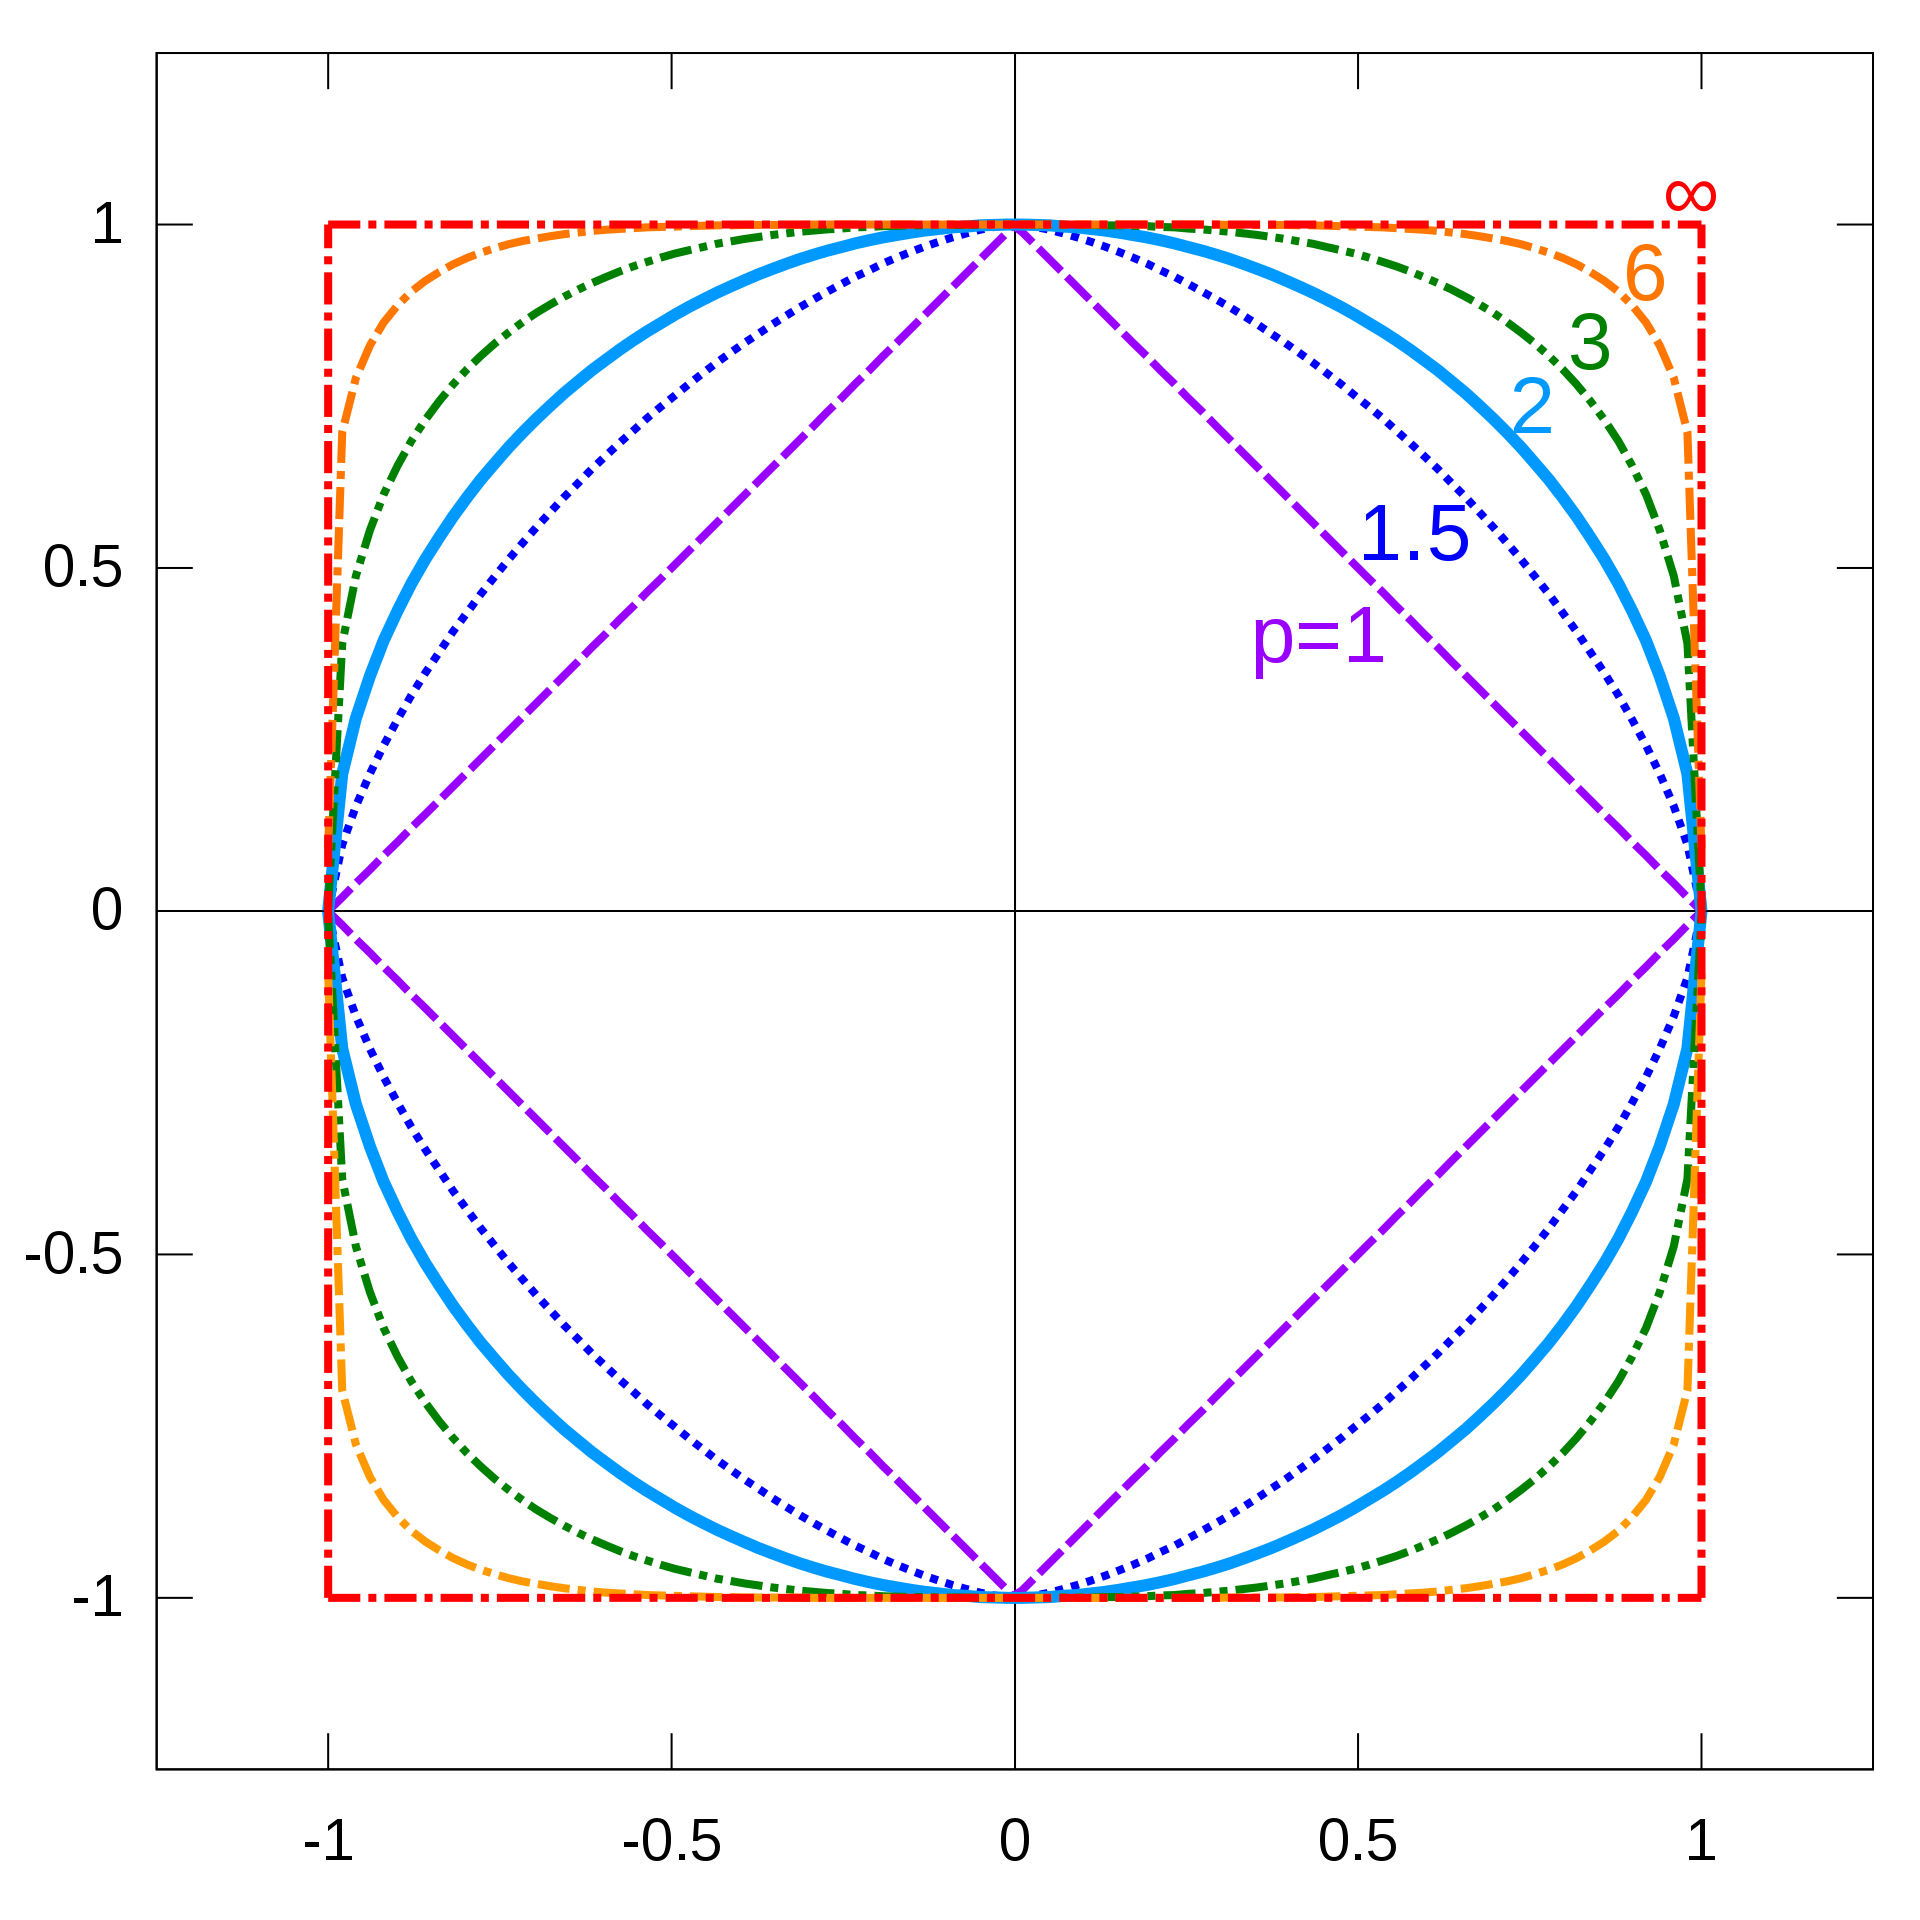
\includegraphics[scale = 0.1]{p-Norms.png}
\end{center}

\end{frame}

\begin{frame}
\frametitle{Inner Products Induce Norms}
If $V$ is an inner product space, the norm induced by the inner product is
$$
\| v\| = \sqrt{\langle v, v\rangle}.
$$
\end{frame}

\begin{frame}[t]
\frametitle{Law of Cosines and Inner Products}
People like to think of inner products defining the angle $\theta$ between vectors
$$
\langle u, v\rangle = \| u\| \|v\|\cos\theta
$$
In particular, we say $u$ and $v$ are {\bf orthogonal} if
$$
\langle u, v\rangle = 0.
$$
\end{frame}

\begin{frame}
\frametitle{Gram-Schmidt Orthogonalization Process}
\begin{Theorem}
If $(v_1, v_2, \ldots, v_n)$ is a sequence of linearly independent vectors in an inner product space $V$, then the sequence $(u_1, u_2,\ldots, u_n)$, defined by
$$
u_1 = v_1\qquad\text{and}\qquad u_k = v_k - \sum_{i = 1}^{k - 1} \frac{\langle v_k, u_i\rangle}{\| u_i\|^2} u_i
$$
for $k = 2, 3,\ldots, n$, is an orthogonal sequence in $V$ with the property that
$$
\text{span}\{u_1, u_2,\ldots, u_n\} = \text{span}\{v_1, v_2,\ldots, v_n\}.
$$
\end{Theorem}

\end{frame}

\begin{frame}[t]
\frametitle{Gram-Schmidt Orthogonalization Process}
\small
\begin{Example}
Orthogonalize the first two vectors of the basis $(1, x, x^2,\ldots)$ for the set of polynomials over $\mathbb{R}$ with inner product
$$
\langle p, q\rangle = \int_{0}^1 p(x)q(x)\ dx.
$$
\end{Example}


\end{frame}

\begin{frame}
\frametitle{Orthogonal Basis}
If $(u_1, u_2,\ldots, u_n)$ is an orthogonal basis of $V$, then for $v$ in $V$ we have
$$
v = \alpha_1 u_1 + \alpha_2 u_2 +\ldots + \alpha_n u_n
$$ 
implies
$$
\alpha_i = \frac{\langle v, u_i\rangle}{\|u_i\|^2}.
$$
\end{frame}

\begin{frame}
\frametitle{Cauchy-Schwarz Inequality}
\begin{Theorem}[Cauchy-Schwarz Inequality]
Suppose $u$ and $v$ are in the inner product space $V$. Then
$$
|\langle u, v\rangle| \leq \|u\| \|v\|.
$$
\end{Theorem}
\end{frame}

\begin{frame}
\frametitle{Distance}
\begin{Definition}
A bivariate function $d$ on a set $V$ is a {\bf distance metric} if for all $u, v, w$ in $V$ the following hold.
\begin{enumerate}
\item[D.1] $d(u, v) \geq 0$ and $d(u, v) = 0$ if and only if $u = v$
\item[D.2] $d(u, v) = d(v, u)$
\item[D.3]  $d(u, v) + d(v, w) \geq d(u, w)$
\end{enumerate}
\end{Definition}
\end{frame}

\begin{frame}
\frametitle{Distance Metric Examples}

\begin{itemize}
\item For the real vector space $\mathbb{R}^n$, the Euclidean distance is most common. Given $x = \left(x_1, x_2, \ldots, x_n\right)$ and $y = (y_1, y_2, \ldots, y_n)$, it is defined to be
$$
d(x, y)= \sqrt{(x_1 - y_1)^2 + (x_2 - y_2)^2 +\ldots + (x_n -y_n)^2}.
$$
\item The discrete metric on any set:
$$
d(x, y) = \begin{cases} 1	&	x \neq y\\ 0	&	x = y.\end{cases}
$$
\item On the set of continuous real-valued functions on the interval [0, 1], we can define
$$
d(f, g) = \int_0^1 \left| f(x) - g(x)\right|\ dx.
$$
\end{itemize}

\end{frame}

\begin{frame}
\frametitle{Norms Induce Distances}
The distance metric induced by a norm is
$$
d(u, v) = \| u - v\|.
$$
\end{frame}


\subsection{Orthogonality and Best Approximation}

\begin{frame}
\frametitle{The Projection Theorem}
\begin{Definition}
The {\bf orthogonal complement} of a set $X\subseteq V$ is the set
$$
X^\perp = \{v \in V: \langle x, v\rangle = 0\ \text{for all}\ x\in X\}.
$$
\end{Definition}

\begin{Theorem}[Projection Theorem]
If $U$ is a finite-dimensional subspace of an inner product space $V$, then for each element $v$ in $V$, there exists unique elements $u$ in $U$ and $u^\perp$ in $U^\perp$ such that
$$
v = u + u^\perp.
$$
\end{Theorem}
\end{frame}

\begin{frame}
\frametitle{Best Approximation}
The Projection Theorem tells us that from $u\; '$ in $U$, we will alway have
$$
\| v - u\| \leq \| v - u\; '\|.
$$

\end{frame}

\begin{frame}[t]
\frametitle{Projection Example}
\begin{Example}
Consider the inner product space of continuous functions on $[0, 1]$, where the inner product is
$$
\langle p, q\rangle = \int_0^1 p(x) q(x)\ dx.
$$
Project $e^x$ onto the subspace spanned by the orthogonal vectors $1$ and $x - 1/2$. Compare the projection with the tangent line approximation at $x = 1/2$.
\end{Example}
\end{frame}

\begin{frame}
\frametitle{Projection Example Solution}
 {\tiny  {\bf Solution.} The projection is
$$
proj(x) = a_{proj}+ b_{proj} \left(x - \frac{1}{2}\right),
$$
where
\begin{align*}
a_{proj}	& = \frac{\langle 1, e^x\rangle}{\|1\|^2}		&	b_{proj} 	&= \frac{\langle x - 1/2, e^x\rangle}{\| x - 1/2 \|^2}\\
		& = \frac{\int_0^1 e^x\ dx}{\int_0^1 1^2\ dx}		&			&= \frac{ \int_0^1 (x - 1/2)e^x\ dx}{\int_0^1 (x - 1/2)^2\ dx} \\
		& = e - 1								&			&=  6(3 - e).
\end{align*}
The tangent line approximation is
$$
tl(x) = a_{tl} + b_{tl} \left(x - \frac{1}{2}\right),
$$
where
$$
a_{tl} = e^{1/2}\qquad b_{tl} = e^{1/2}.
$$
}

\end{frame}

\begin{frame}[fragile]
\frametitle{Projection Example Solution Python Code}
{
\linespread{0.8}
\tiny
\begin{verbatim*}
import numpy as np, matplotlib.pyplot as plt
from scipy.integrate import quad

# Use Seaborn style
plt.style.use('seaborn')

# Define norm
inner = lambda f, g: quad(lambda x: f(x) * g(x), 0, 1)[0]

# Define basis elements
u1, u2 = lambda x: 1, lambda x: x - 1/2 

# Calculate inner products
a_proj, b_proj = inner(u1, np.exp)/inner(u1, u1), inner(u2, np.exp)/inner(u2, u2) 

# Define small value
h = 1e-5

# Calculate tangent line coeffs
a_tl, b_tl = np.exp(1/2), (np.exp(0.5 + h) - np.exp(0.5 - h))/(2 * h)

# Define functions 
proj, tl = lambda x: a_proj * u1(x) + b_proj * u2(x), lambda x: a_tl * u1(x) + b_tl * u2(x)

# Get the x-values for plot
x_vals = np.linspace(0, 1, 100)

# Plot results
plt.plot(x_vals, [proj(x) for x in x_vals], label = 'Projection')
plt.plot(x_vals, [tl(x) for x in x_vals], label = 'Tangent Line')
plt.plot(x_vals, [np.exp(x) for x in x_vals], label = 'True')
# Create a legend
plt.legend()
# Save the figure
plt.savefig(r'[location on machine]')
# Show plot
plt.show()
\end{verbatim*}
}
\end{frame}

\begin{frame}[fragile]
\frametitle{Projection Example Image}
\begin{center}
\includegraphics[scale = 0.5]{ex6.png}
\end{center}
\end{frame}

\begin{frame}[fragile]
\frametitle{Projection Example Solution Result}
{
\linespread{0.8}
\tiny
\begin{verbatim*}
# Define norm
norm = lambda f: np.sqrt(inner(f, f))

# Let's calculate the norms
norm_proj, norm_tl = norm(lambda x: np.exp(x) - proj(x)), norm(lambda x: np.exp(x) - tl(x))

print(f'Using the projection approximationmthe norm is {norm_proj:.3f}.')
print(f'Using the tangent line approximation the norm is {norm_tl:.3f}.')\end{verbatim*}
}
The output reads:
\begin{quote}
{
\small
\texttt{Using the projection approximationmthe norm is 0.063.}\\
\texttt{Using the tangent line approximation the norm is 0.094.}
}
\end{quote}
\end{frame}



\end{document}
